\section{Experimental Evaluation} \label{subsec:setup}

Our data set consists of 148 process descriptions annotated by a biologist. The annotator was presented with annotation guidelines and annotated 20 descriptions. The annotations were then discussed with the authors, after which all process descriptions were annotated. After training a second biologist, we measured inter-annotator agreement $\kappa=0.69$, on 30 random process descriptions. 

Process descriptions were parsed with Stanford constituency and dependency parsers \cite{Klein03,Marneffe06}, and 35 process descriptions were set aside as a test set (\# of training set trigger pairs: 1932, \# of test set trigger pairs: 906). We performed 10-fold cross validation over the training set for feature selection and tuning of constraint parameters. For each constraint type (connectivity, chain-structure, and five triad constraints) we introduced a parameter and tuned the seven parameters by coordinate-wise ascent, where for hard constraints a binary parameter controls whether the constraint is used, and for soft constraints we attempted 10 different reward/penalty values. Last, for our global model we defined $\theta_{ijr}=\log p_{ijr}$, where $p_{ijr}$ is the marginal probability at edge $(i,j)$ of label $r$.


We test the following systems: (a) \emph{All-Prev}: Since the most common process structure was chain-like, we simply predict \textsc{Prev} for every two adjacent triggers in text. (b) \emph{Local$_{base}$}: A pairwise classifier with features from previous work (Section~\ref{subsec:pairwise}) (c) \emph{Local}: A pairwise classifier with all features (Section~\ref{subsec:pairwise-novel}) (d) \emph{Global}: Our full model that uses ILP inference.

%(d) \emph{Local$_{chain}$}: For every two adjacent triggers we pick the highest probability non-\textsc{None} relation using the local classifier. Again, this uses the assumption that many processes have a chain-structure.

To evaluate system performance we compare the set of predictions on all trigger pairs to the gold standard annotations and compute micro-averaged precision, recall and F$_1$. We perform two types of evaluations: (a) \emph{Full}: evaluation on our full set of 11 relations (b) \emph{Temporal:} Evaluation on temporal relations only, by collapsing \textsc{Prev}, \textsc{Causes}, and \textsc{Enables} to a single category and similarly for \textsc{Next}, \textsc{Caused}, and \textsc{Enabled} (inter-annotator agreement $\kappa=0.75$). We computed statistical significance of our results with the paired bootstrap resampling method \cite{efron1993}.

\subsection{Results} \label{subsec:results}

\begin{table}[t]
\setlength{\tabcolsep}{5pt}
{\footnotesize
\begin{tabular}{  l | l  l  l | l  l  l  }
%\hline
    & \multicolumn{3}{c|}{\textbf{Temporal}} & \multicolumn{3}{c}{\textbf{Full}} \\
    & P & R & F$_1$ & P & R & F$_1$ \\
%\hline
\hline
\emph{All-Prev} & 58.4 & 54.8 & 56.6 & 34.1 & 32.0 & 33.0 \\
\emph{Local$_{base}$} & 61.5 & 51.8 & 56.2 &  52.1 & 43.9 & 47.6\\
\emph{Local} & 63.2 & 55.7 & 59.2 & 54.7 & 48.3 & 51.3 \\
\emph{Global} & \textbf{63.9} & \textbf{61.4$^{\dagger\ddagger}$} & \textbf{62.6$^{\dagger\ddagger}$} & \textbf{56.2} & \textbf{54.0$^{\dagger\ddagger}$} & \textbf{55.0$^{\dagger\ddagger}$} 
%\hline
\end{tabular}}
\caption{Test set results on all experiments. Best number in each column is bolded. $\dagger$ and $\ddagger$ denote statistical significance ($p<0.01$) against \emph{Local$_{base}$} and \emph{Local} baselines, respectively.}
\label{tab:results}
\end{table}

Table~\ref{tab:results} presents performance of all systems. We see that using global constraints improves performance on all measures in both full and temporal evaluations. Particularly, in the full evaluation recall improves by 12\% and overall F$_1$ improves significantly by 3.7 points against \emph{Local} ($p<0.01$). Recall improvement suggests that modeling connectivity allowed \emph{Global} to add correct relations in cases where some events were not connected to one another.

The \emph{Local} classifier substantially outperforms \emph{Local$_{base}$}. This indicates that our novel features (Section~\ref{subsec:pairwise-novel}) are important for discriminating between process relations. Specifically, in the full evaluation \emph{Local} improves precision more than in the temporal evaluation, suggesting that designing syntactic and semantic features for connectives is useful for distinguishing \textsc{Next}, \textsc{Causes}, and \textsc{Enables} when the amount of training data is small.

The \emph{All-Prev} baseline performs badly in the full evaluation, but in temporal evaluation it works reasonably well. This demonstrates that process descriptions tend to proceed linearly from one event to the other, which is a known property of discourse structure \cite{schegloff73}.

Table~\ref{tab:degree} presents the degree distribution of \emph{Local} and \emph{Global} on the development set comparing to the gold standard. Clearly, degree distribution of \emph{Global} is much more similar to the gold standard than \emph{Local}. In particular, the connectivity constraint ensures that there are no isolated nodes and shifts mass from nodes with degree $0$ and $1$ to nodes with degree $2$.

Table~\ref{tab:paramtuning} presents the order in which global constraints were introduced into the model using coordinate ascent on the development set. Connectivity is the first constraint to be introduced, and improves performance considerably. The chain constraint, on the other hand, is included third and the improvement in F$_{1}$ score is relatively smaller. This can be explained by the distribution of degrees in Table~\ref{tab:degree} which shows that the predictions of \emph{Local} does not have many nodes with degree $>2$. As for triad constraints, we see that four constraints are important and are included in the model, but one is discarded.

\begin{table}[t]
{\footnotesize
\begin{tabular}{ l | l | l | l }
%\hline
    \textbf{Order} & \textbf{Parameter name} & \textbf{Value} ($\alpha$)& \textbf{F$_1$ score} \\
%\hline
\hline
- & \emph{Local model} & - & 49.9 \\
1 & Connectivity constraint & $\infty$ & 51.2 \\
2 & \textsc{Same} transitivity &  0.5 & 52.9 \\
3 & Chain constraint & -0.5 & 53.3\\
4 & \textsc{Cause}-\textsc{Cotemp} & 1.0 & 53.7\\
6 & \textsc{Prev} contradiction & $\infty$ & 53.8\\
7 & \textsc{Same} contradiction & $\infty$ & 53.9
%\hline
\end{tabular}}
\caption{Order by which constraint parameters were set using coordinate ascent on the development set. For each parameter, the value chosen and F$_1$ score after including the constraint are provided. Negative values correspond to penalties, positive values to rewards, and a value of $\infty$ indicates a hard constraint.}
\label{tab:paramtuning}
\end{table}

\subsection{Qualitative Analysis} \label{subsec:analysis}
\begin{figure*}[t]
\centering
\fbox{ 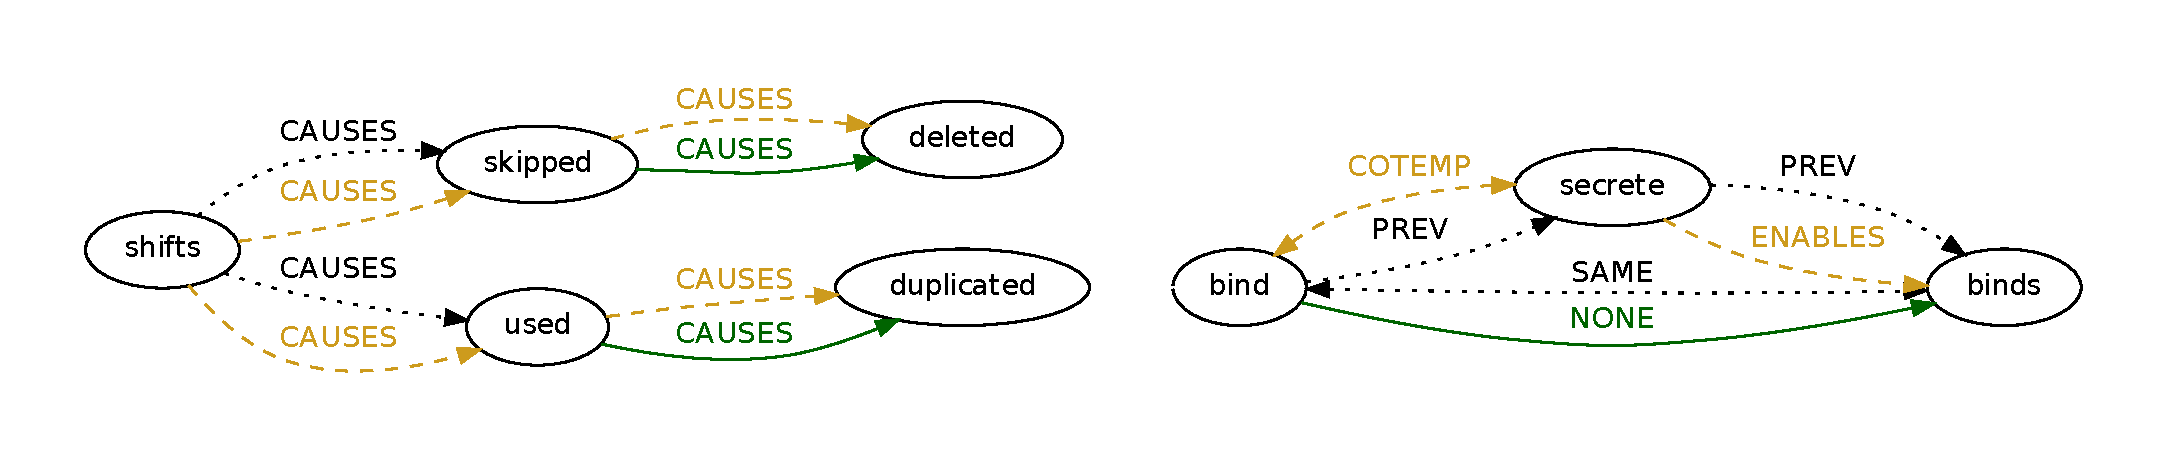
\includegraphics[width=0.98\textwidth]{figures/example}}
\caption{Fragments of process graphs. Black edges (dotted) are predictions of \emph{Local}, green edges (solid) indicate edges modified by \emph{Global}, and gold edges (dashed) represent gold standard edges. Original text, Left: ``... the template \emph{shifts} with respect to the new complementary strand, and a part of the template strand is either \emph{skipped} by the replication machinery or \emph{used} twice as a template.
As a result, a segment of DNA is \emph{deleted} or \emph{duplicated}." Right: ``Cells of mating type A secrete a signaling molecule, which can \emph{bind} to specific receptor proteins on nearby cells. At the same time, cells \emph{secrete} factor, which \emph{binds} to receptors on a cells."}
\label{fig:graph}
\end{figure*}

Figure~\ref{fig:graph} shows two examples where global constraints corrected the predictions of \emph{Local}. In Figure~\ref{fig:graph}, left, \emph{Local} failed to predict the causal relations \emph{skipped}-\emph{deleted} and \emph{used}-\emph{duplicated}, possibly because they are not in the same sentence and are not adjacent to one another. By enforcing the connectivity constraint, \emph{Global} correctly connects \emph{deleted} and \emph{duplicated} to the other triggers in the process.

In Figure~\ref{fig:graph}, right, \emph{Local} predicts a structure that results in a ``\textsc{Same} contradiction" structure. The triggers \emph{bind} and \emph{binds} cannot denote the same event if a third trigger \emph{secrete} is temporally between them. However, since \emph{bind} and \emph{binds} share the same lemma, \emph{Local} predicts that they are co-referring triggers. \emph{Global} prohibits this structure and correctly predicts the relation as \textsc{None}.

To better understand the performance of \emph{Local}, we analyzed the confusion matrix generated based on its predictions. Although this is a challenging 11-class classification task, most of the mass is concentrated on the matrix diagonal, as desired. Error analysis reveals that 17.5\% of all errors are confusions between \textsc{None} and \textsc{Prev}, 11.1\% between \textsc{Prev} and \textsc{Causes}, and 8.6\% between \textsc{Prev} and \textsc{Cotemp}. This demonstrates that distinguishing the classes \textsc{Prev}, \textsc{Causes} and \textsc{Cotemp} is challenging for \emph{Local}. Our current global constraints do not address this type of error, and thus an important direction for future work is to improve the local model. 

The global model depends on the predictions of the local classifier, and so enforcing global constraints does not guarantee improvement in performance. For instance, if \emph{Local} produces a graph that is disconnected (e.g, \emph{deleted} in Figure~\ref{fig:graph}, left), then \emph{Global} will add an edge. However, the label of the edge is determined by the local classifier, and if this prediction is wrong we will now be penalized both for the false negative of the correct class (just as before) but also for the false positive of the predicted class.  Despite that we see that \emph{Global} improves overall performance by 3.7 F$_{1}$ points on the test set.
